\documentclass{beamer}
% \usetheme{Darmstadt}
% \usetheme{Antibes}
\usetheme{Berlin}
\usepackage{svg}
% \usepackage{graphicx} % Required for inserting images

\definecolor{IUgreen}{RGB}{64, 186, 33}
\definecolor{IUgreylight}{RGB}{237, 241, 245}
\definecolor{IUgreytext}{RGB}{51, 51, 51}
\definecolor{IUgrey}{RGB}{145, 163, 176}

\setbeamercolor{palette primary}{bg=IUgreen,fg=white}
\setbeamercolor{palette secondary}{bg=IUgreylight,fg=IUgreytext}
\setbeamercolor{palette tertiary}{bg=IUgreen,fg=white}
\setbeamercolor{palette quaternary}{bg=IUgreen,fg=white}
\setbeamercolor{structure}{fg=IUgreen} % itemize, enumerate, etc
\setbeamercolor{section in toc}{fg=IUgreen} % TOC sections
% \setbeamercolor{navigation symbols}{fg=IUgreytext}
% \setbeamercolor{navigation symbols dimmed}{fg=IUgrey}

\usepackage{hyperref}
\usepackage{xcolor}
\usepackage{multicol}

\title{Accelerated Gradient Clipping}
\subtitle{Optimization Methods in Machine Learning}
\author{Danil Andreev \and Vladimir Makharev}
\institute{Innopolis University}
\date{Fall 2023}

\begin{document}

\begin{frame}
    \titlepage
    \begin{figure}[htpb]
        \begin{center}
            \includesvg[height=0.06\linewidth]{pics/iu_logo_green_eng.svg}
        \end{center}
    \end{figure}
\end{frame}

\section{Gradient Clipping}
\begin{frame}
    \frametitle{Gradient clipping}
    $$\text{clip}\left(\nabla f(x, \xi), \lambda \right) = \min \left\{1, \frac{\lambda}{||\nabla f(x, \xi)||} \right\} \nabla f(x, \xi)$$

    \begin{itemize}
        \item $\nabla f(x, \xi)$ - stochastic gradient of the objective function at point $x$
        \item $\lambda$ - clipping parameter, larger $\lambda$ means less aggressive clipping
        \item $||\nabla f(x, \xi)||$ - Euclidean norm of the gradient vector
    \end{itemize}

    As a result, the gradient vector is projected on the Euclidean ball with radius $\lambda$ with center at the origin.
\end{frame}

\begin{frame}
    \frametitle{Gradient clipping}
    \begin{itemize}
        \item In SGD, mini-batches are used for gradient computation.
        \item These mini-batches introduce randomness, leading to high-variance gradient estimates.
        \item Gradient clipping helps stabilize training by preventing extreme updates caused by these fluctuations.
    \end{itemize}
\end{frame}


\section{Paper Experiments}
\begin{frame}
    \frametitle{SGD and SSTM trajectories on \texttt{diabetes} dataset}
    \begin{multicols}{2}
        \noindent
        \includesvg[width=\linewidth]{pics/paper_experiments/diabetes_sgd.svg} \par
        \includesvg[width=\linewidth]{pics/paper_experiments/diabetes_sstm.svg}
    \end{multicols}
\end{frame}

\begin{frame}
    \frametitle{SGD trajectories on \texttt{australian} dataset}
    \begin{figure}[htpb]
        \begin{center}
            \includesvg[width=0.8\linewidth]
                {pics/paper_experiments/australian_sgd.svg}
        \end{center}
    \end{figure}
\end{frame}

\begin{frame}
    \frametitle{SGD and SSTM trajectories on \texttt{heart} dataset}
    \begin{multicols}{2}
        \noindent
        \includesvg[width=\linewidth] {pics/paper_experiments/heart_sgd.svg} \par
        \includesvg[width=\linewidth] {pics/paper_experiments/heart_sstm.svg}
    \end{multicols}
\end{frame}


\section{Experiments}
\begin{frame}
\frametitle{Fine-tuning BERT on Yelp reviews}
We built a pipeline to fine-tune a pretrained model based on \href{https://huggingface.co/docs/transformers/training#train-in-native-pytorch}{\color{blue}HuggingFace docs}
\begin{itemize}
    \item Pretrained BERT (\texttt{bert-base-cased}) model
    \item \href{https://huggingface.co/datasets/yelp_review_full}{\color{blue}Yelp reviews} dataset of text reviews and score between 1 and 5
    \item Dataset splits: \texttt{(train, val, eval) = (1000, 300, 500)}
\end{itemize}
\only<2->{Hyperparameters:}
\begin{itemize}
    \item<2-> \texttt{batch\_size = 8}
    \item<2-> \texttt{num\_epochs = 3}
    \item<2-> \texttt{learning\_rate = 0.00005}
\end{itemize}
\end{frame}

\begin{frame}
\frametitle{Experiments with BERT fine-tuning on optimizers}
We experimented with \href{https://pytorch.org/docs/stable/optim.html}{\color{blue}PyTorch optimizers} SGD and AdamW. For clipping, \href{https://github.com/pytorch/pytorch/blob/0597eb56c29b3986aa412161b1d3e82b6b36e8d5/torch/nn/utils/clip_grad.py#L12}{\color{blue}\texttt{clip\_grad\_norm\_}} function with \texttt{max\_norm}\(\ =\lambda=1.0\) was used. We used \href{https://wandb.ai/makharev/iu-omml}{\color{blue}WandD} to track loss and accuracy. For loss \texttt{smoothing = 0.9} was applied. We denoted momentum as \(\mu\). 
\begin{itemize}
    \item \texttt{SGD}
    \item \texttt{clipped-SGD}
    \item \texttt{SGD} (\(\mu=0.9\))
    \item \texttt{clipped-SGD} (\(\mu=0.9\))
    \item \texttt{SGD-Nesterov} (\(\mu=0.9\))
    \item \texttt{clipped-SGD-Nesterov} (\(\mu=0.9\))
    \item \texttt{AdamW}
    \item \texttt{clipped-AdamW}
\end{itemize}
\end{frame}

\begin{frame}
    \frametitle{Training loss trajectories (\texttt{train} split)}
    \texttt{SGD}, \texttt{clipped-SGD}, \texttt{AdamW}, \texttt{clipped-AdamW}
    \begin{figure}[htpb]
        \begin{center}
            \includegraphics[width=\linewidth]
                {pics/experiments/train_loss_adam_sgd}
        \end{center}
    \end{figure}
\end{frame}

\begin{frame}
    \frametitle{Training loss trajectories (\texttt{train} split)}
    With \(\mu=0.9\): \texttt{SGD}, \texttt{clipped-SGD}
    \begin{figure}[htpb]
        \begin{center}
            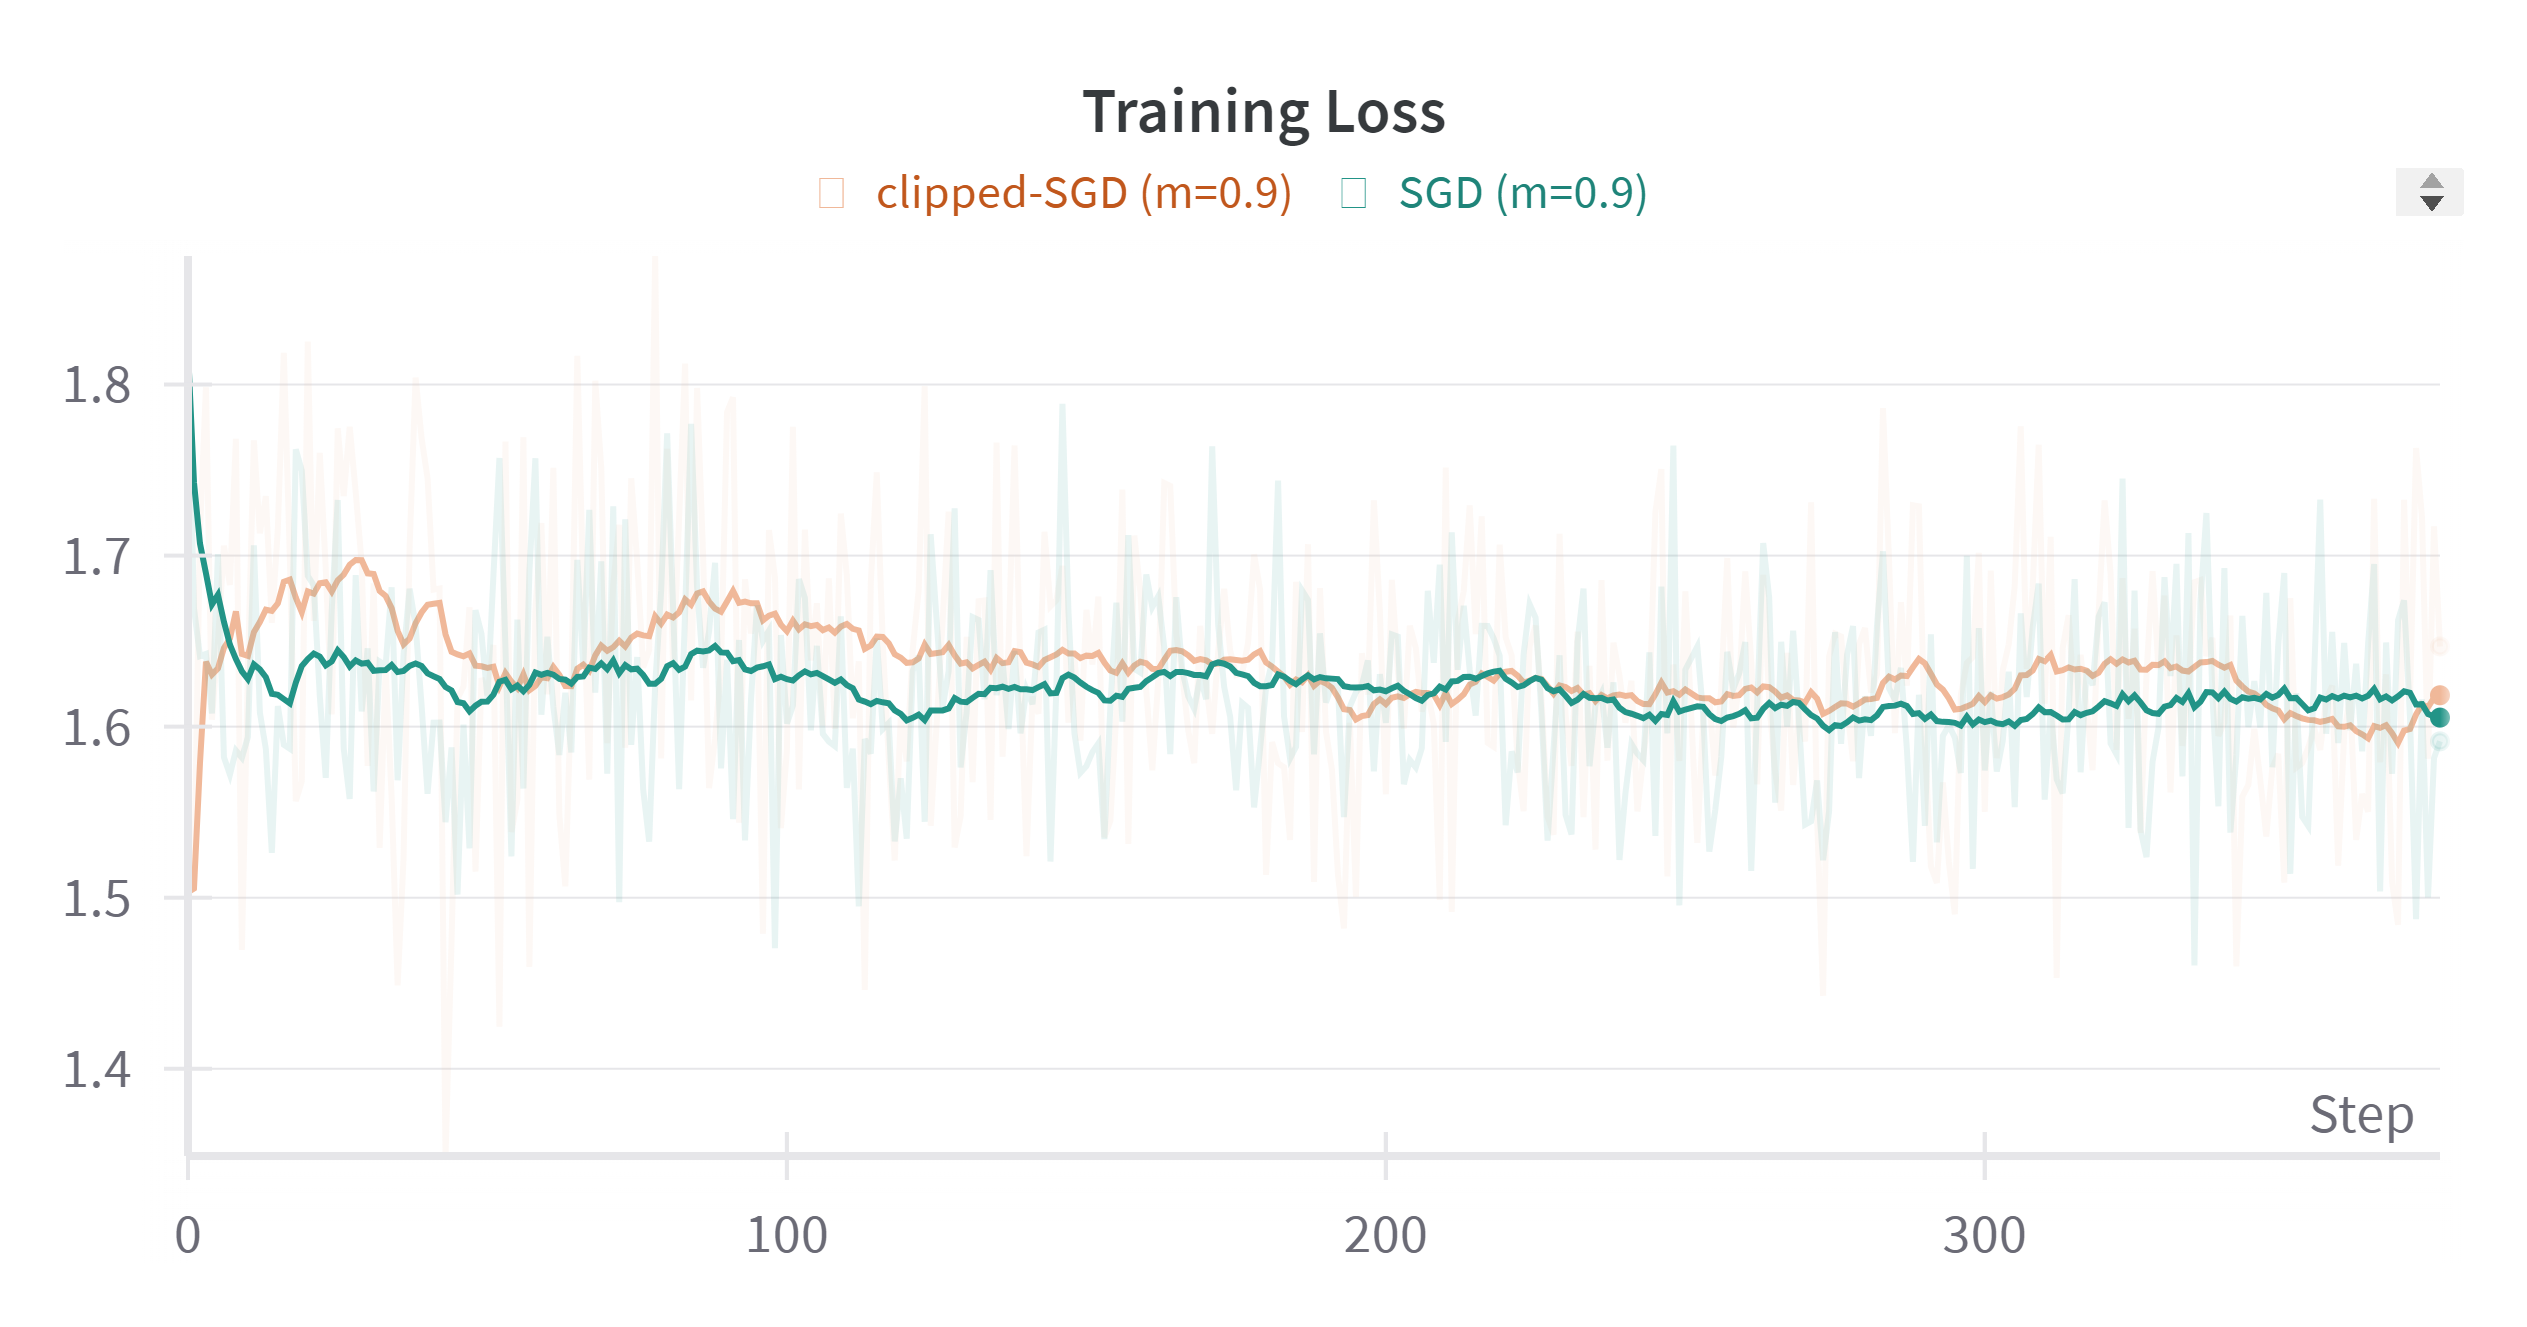
\includegraphics[width=\linewidth]
                {pics/experiments/train_loss_sgdm}
        \end{center}
    \end{figure}
\end{frame}

\begin{frame}
    \frametitle{Training loss trajectories (\texttt{train} split)}
    With \(\mu=0.9\): \texttt{SGD-Nesterov}, \texttt{clipped-SGD-Nesterov}
    \begin{figure}[htpb]
        \begin{center}
            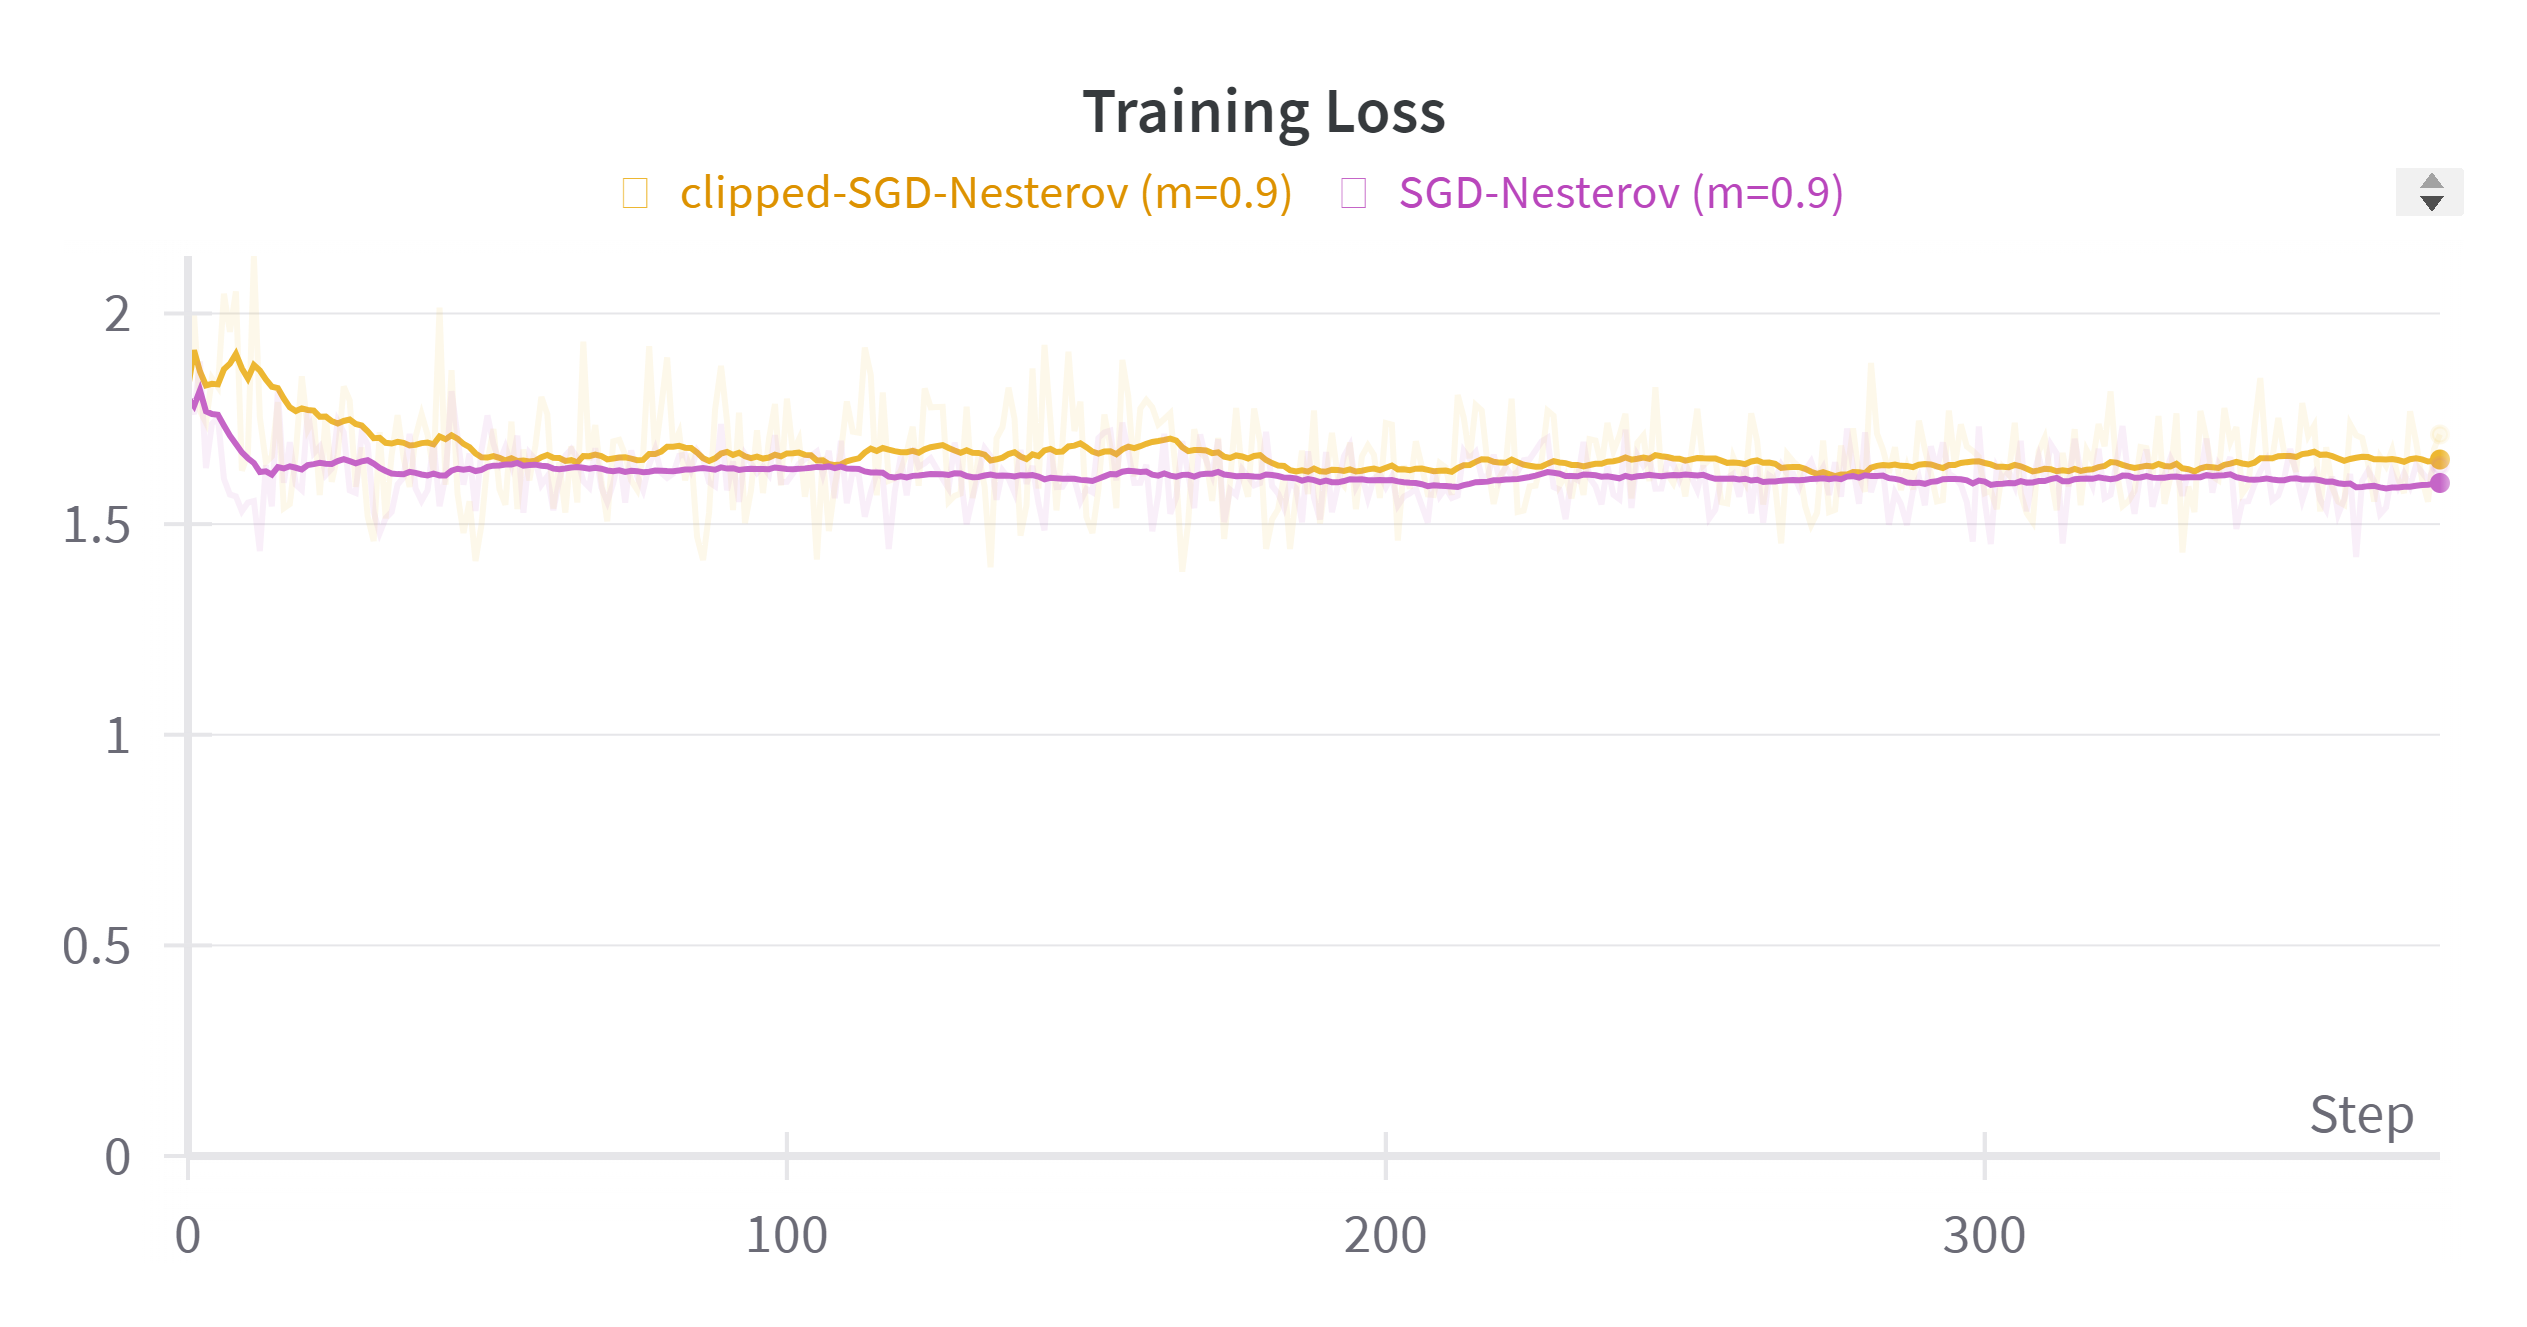
\includegraphics[width=\linewidth]
                {pics/experiments/train_loss_sgdnm}
        \end{center}
    \end{figure}
\end{frame}

\begin{frame}
    \frametitle{Validation accuracy trajectories (\texttt{val} split)}
    \texttt{SGD}, \texttt{clipped-SGD}, \texttt{AdamW}, \texttt{clipped-AdamW}
    \begin{figure}[htpb]
        \begin{center}
            \includegraphics[width=\linewidth]
                {pics/experiments/val_accuracy_good}
        \end{center}
    \end{figure}
\end{frame}

\begin{frame}
    \frametitle{Validation accuracy trajectories (\texttt{val} split)}
    With \(\mu=0.9\): \texttt{SGD}, \texttt{clipped-SGD}, \texttt{SGD-Nesterov}, \texttt{clipped-SGD-Nesterov}
    \begin{figure}[htpb]
        \begin{center}
            \includegraphics[width=\linewidth]
                {pics/experiments/val_accuracy_bad}
        \end{center}
    \end{figure}
\end{frame}

\begin{frame}
    \frametitle{Evaluation accuracy trajectories (\texttt{test} split)}
    \begin{figure}[htpb]
        \begin{center}
            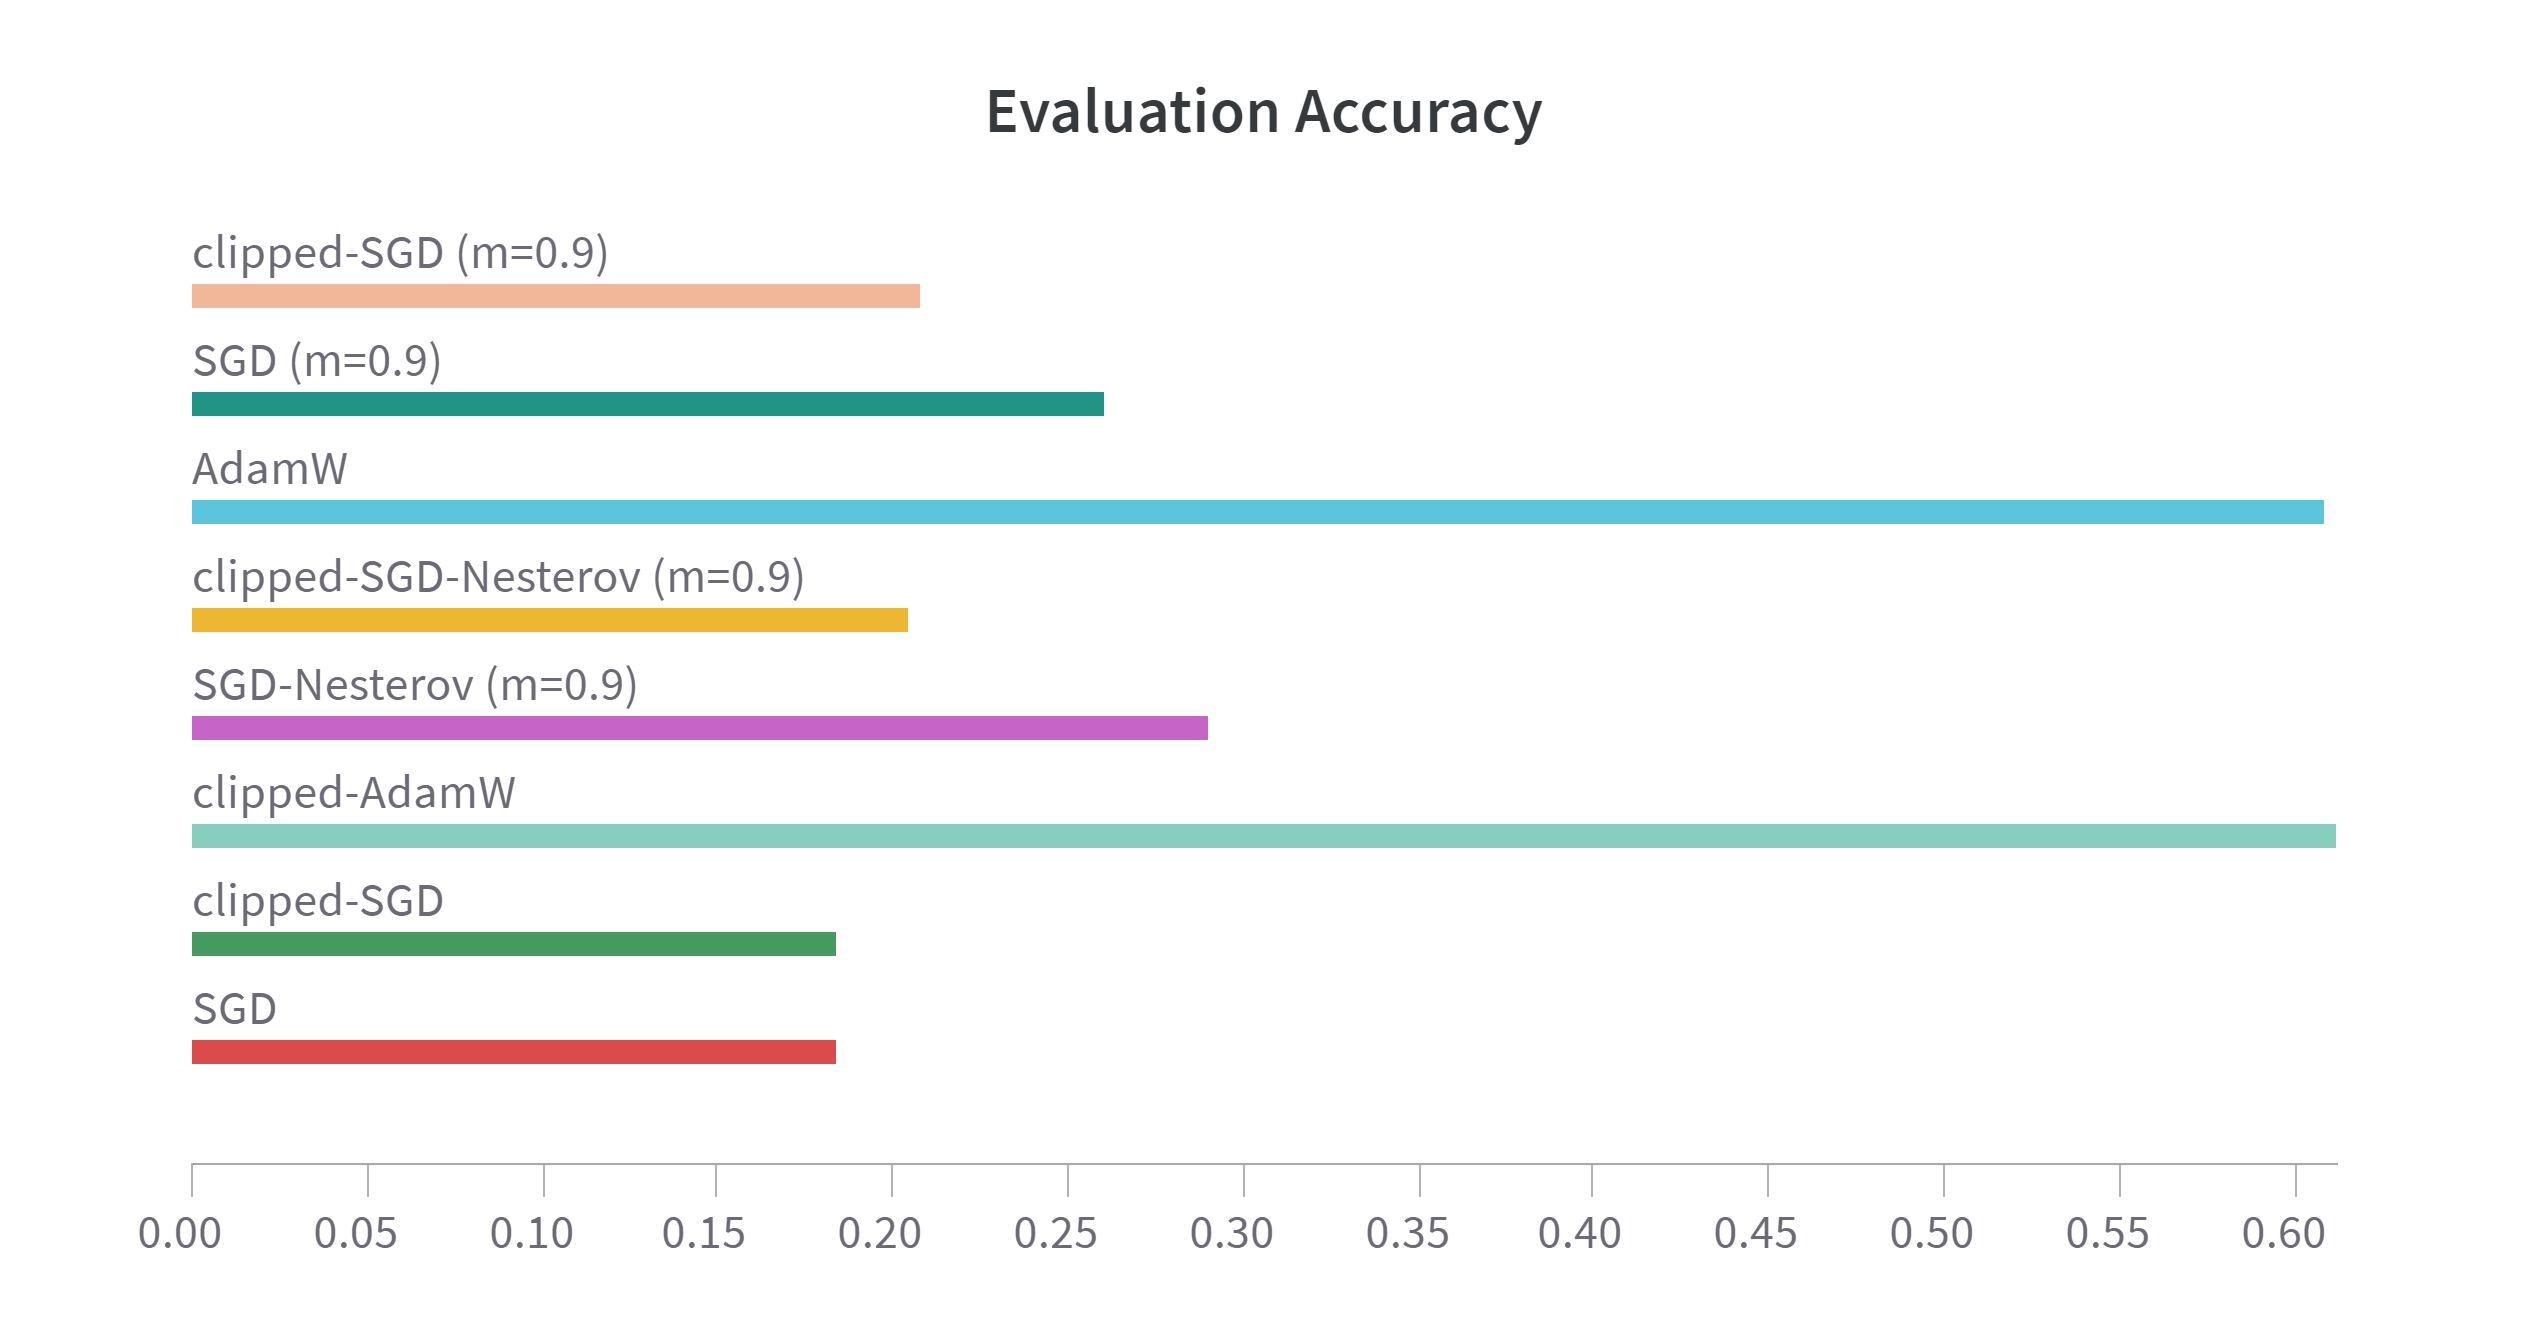
\includegraphics[width=\linewidth]
                {pics/experiments/eval_accuracy}
        \end{center}
    \end{figure}
\end{frame}


\section{Conclusion}
\begin{frame}
\frametitle{Conclusion}
\begin{itemize}
    \item Accelerated gradient clipping in stochastic optimization significantly enhances performance in the presence of heavy-tailed noise
    \item First high-probability complexity bounds (on a number of oracle calls) were derived by authors for \texttt{clipped-SSTM} and \texttt{clipped-SGD} methods
    \item Experiments from paper are easily reproducible
    \item Our experiments in NLP domain shows noticeable improvement in loss convergence for AdamW optimizer with clipping, while for SGD variants optimizers clipping effect is not significant
\end{itemize}
\end{frame}


\section{Appendix}
\begin{frame}
    \frametitle{Preliminaries}
    \begin{figure}[htpb]
        \begin{center}
            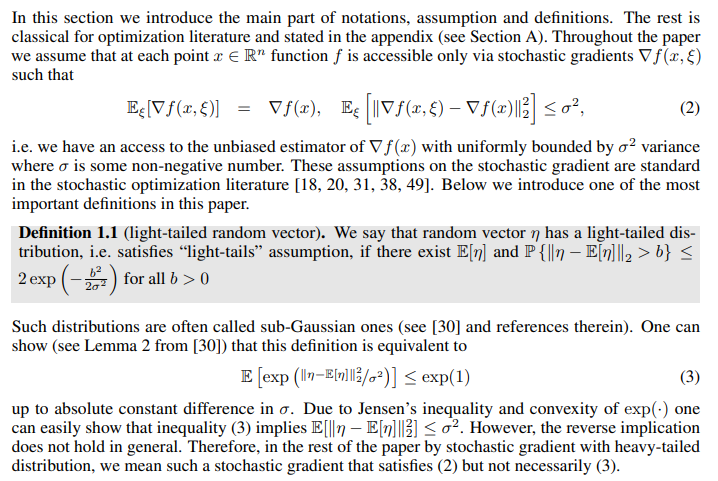
\includegraphics[width=0.9\linewidth]
                {pics/appendix/preliminaries}
        \end{center}
    \end{figure}
\end{frame}

\begin{frame}
    \frametitle{Complexity bounds for convex objectives}
    \begin{figure}[htpb]
        \begin{center}
            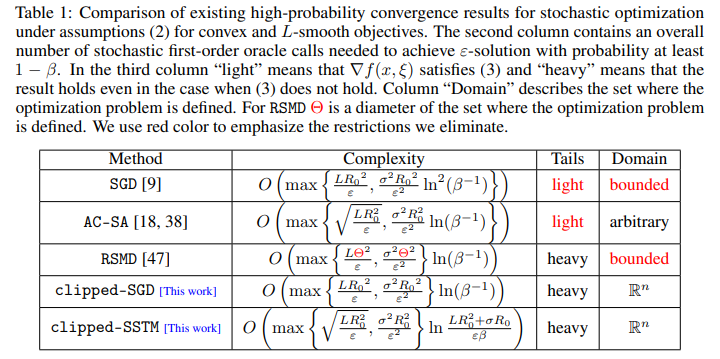
\includegraphics[width=\linewidth]
                {pics/appendix/table_1}
        \end{center}
    \end{figure}
\end{frame}

\begin{frame}
    \frametitle{Complexity bounds for \(\mu\)-strongly convex objectives}
    \begin{figure}[htpb]
        \begin{center}
            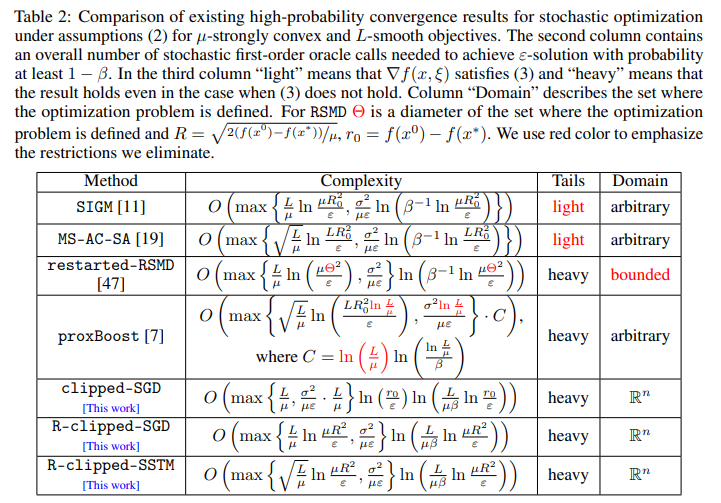
\includegraphics[width=0.9\linewidth]
                {pics/appendix/table_2}
        \end{center}
    \end{figure}
\end{frame}


\end{document}
